\chapter{Laplace Transforms}

\section{Solving ODEs using Laplace Transform}

\begin{weekintro}
  \begin{fullwidth}
  Functions that represent solutions of differential equations can be given a formula (\emph{representation}) in time-domain, where it's very easy to interpret their values/graph them, or in \index{Laplace!transform} Laplace domain\index{Laplace!domain}, where it is very easy to manipulate them through derivatives and integrals.\index{Laplace transform!derivative}

  Notice that even though \(f(t)\) is a real valued function of a real number, its Laplace transform\index{Laplace transform} \(F(s)\) is a complex-valued function of a complex-number. That means that \(f(t)\) can be visualized as a curve over a real axis, but we run into problems when visualizing \(F(s)\). The domain is a complex plane \(s \in \mathbb{C}\) but what do we put on ``height'' axis above this plane?\index{complex-valued functions}

  The value of \(F(s)\) is a complex number itself, requiring either real/imaginary or modulus/argument representation, so we have to choose which component to plot as ``height''. At this point, it's illustrative to visualize \(\abs{F(z)}\) and \(\arg F(z)\) separately in some way.

  The \sage code \url{https://goo.gl/2H2uBF} visualizes a function \(f(t) = e^{-2t}\) in three different ways:
  \begin{inparaenum}[(i)]
  \item as ``usual'' in time-domain,
  \item magnitude of its Laplace transform \(\abs{F(s)}\) in 3d,
  \item its Laplace transform as brightness (\(\abs{F(s)}\)) and color (\(\arg F(s)\)).
  \end{inparaenum}
  If you visit the link you can also rotate the 3d graph, show angle, real, and imaginary parts of \(F(s)\).
  % \begin{figure}
  %   \begin{subfigure}{0.33\linewidth}
  %     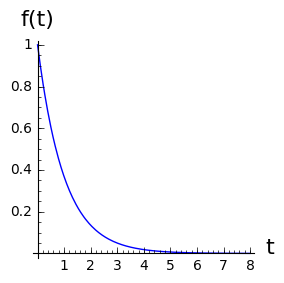
\includegraphics[height=1.5in]{figs/time-domain}
  %     \caption{\(f(t)\)}
  %   \end{subfigure}\hfill
  %   \begin{subfigure}{0.33\linewidth}
  %     \includegraphics[height=1.5in]{figs/laplace-domain-2d.png}
  %     \caption{\(\abs{F(s)}\) is brightness, \(\arg F(s)\) is color, \\axes are \(\Re s\) and \(\Im s\)  }
  %   \end{subfigure}\hfill
  %   \begin{subfigure}{0.33\linewidth}
  %     \includegraphics[height=1in]{figs/laplace-domain-3d}
  %     \caption{\(\abs{F(s)}\) is height, \\axes are \(\Re s\) and \(\Im s\) }
  %   \end{subfigure}
  %   \caption{\(f(t)\) and the corresponding \(F(s)\) plotted by \url{https://goo.gl/2H2uBF}}
  % \end{figure}

  Notice that the decay\index{decay} rate \(-2\) from \(f(t)\) translates into points where \(\abs{F(s)}\) grows \index{growth} very large (diverges). At the same time, the color around \(s = -2 + 0i\) rotates through the full color spectrum, indicating that its angle (argument) changes around that point.
\end{fullwidth}
\end{weekintro}
\subsection*{Homework}

\begin{sagequestion}
  Modify the line 6 in  \url{https://goo.gl/2H2uBF} to visualize \(f(t) = e^{-t}\cos(2t)\) and use the outputs to answer the following questions.
  \begin{enumerate}[(a)]
  \item \(F(s) = \) \solspace{0.25in}
  \item Sketch the graph of absolute value \(\abs{F(s)}\).
  \item Use the 3d and 2d color graph\footnote{If you find these graphs interesting, there are many more in the gallery at \url{http://www.visual.wegert.com/}.} to determine distinguished values where \(\abs{F(s)}\)

    Blows up: \hspace{2in} Goes to zero: \hspace{2in}

  \item By hand, calculate the (complex) roots of the denominator of \(F(s)\). Roots =

    How do they relate to your answer in previous item? \solspace{0.25in}
  \end{enumerate}


\end{sagequestion}
\newpage
\begin{question}
  Use the\index{Laplace!integral} integral Laplace formula\footnote{ Laplace transforms:

    \(
    \begin{aligned}
    \laplace\braced{f} &= \int_{0}^{\infty} e^{-st} f(t)dt  \\
    \laplace^{-1}\braced{F} &= \int_{0}^{\infty} e^{st} F(s)ds
  \end{aligned}
    \)
  }  to compute
  \(
    \laplace\braced*{7 t^{2}}
    \) (hint: use repeated integration-by-parts).\index{integration!by parts}
    \solspace{2in}
  \end{question}

  \begin{question}
    Use table conversions\footnote{The Laplace table is in the appendix.} to compute the following Laplace transforms:
    \begin{enumerate}[(a)]
    \item \(\laplace\braced*{e^{-3t} + 4+2t} \) \solspace{1in}
    \item \(\laplace\braced*{3 \sin(4t)} \) \solspace{1in}
    \item \(\laplace\braced*{3 e^{3t}\sin(4t)} \) \solspace{1in}
    \end{enumerate}
  \end{question}

  \begin{question}
    Use table conversions\footnote{The Laplace table is in the appendix.} to compute the following inverse Laplace transforms:\index{partial fractions}
    \begin{enumerate}[(a)]
    \item \(\laplace^{-1}\braced*{\frac{3}{s+2}} \) \solspace{1in}
    \item \(\laplace^{-1}\braced*{\frac{2}{s^{2} + 9}} \) \solspace{1in}
    \item \(\laplace^{-1}\braced*{\frac{s+5}{ s^{2} + 2s + 5}} \) \solspace{2in}
    \end{enumerate}
  \end{question}

  \begin{question}
    Solve the following IVPs using the Laplace transform\footnote{Make sure to use the derivative rule:\(\laplace\braced{y'(x)} = s\laplace\braced{y(x)} - y(0)\)}:
    \begin{enumerate}[(a)]
    \item \(y'(x) + 2y(x) = e^{-3x}, \quad y(0) = 5\)\solspace{3in}
    \item \(y''(x) + 2y'(x) + 5y(x) = 0 \quad y(0) = 0, y'(0)=1\)\solspace{3in}
    \end{enumerate}
  \end{question}


\subsection*{Discussion Problems}

\begin{question}
Find the Laplace transforms using the table and rules:
\begin{enumerate}[(a)]
  \item $\laplace\braced*{5t^4-2e^{5t}}$
  \item $\laplace \braced*{ \cos(5t)+\sin(2t) }$
  \end{enumerate}
\end{question}

\begin{question}
Find the inverse Laplace transforms using the table and rules:
 \begin{enumerate}[(a)]
 \item $\laplace^{-1}\braced*{ \frac{1}{s^3} }$
 \item $\laplace^{-1}\braced*{\frac{1}{s^2}-\frac{1}{s} +\frac{1}{s+2} -\frac{1}{s-2}}$
 \item $\laplace^{-1}\braced*{\frac{10s}{s^2+16}}$
 \item $\laplace^{-1}\braced*{\frac{2s-4}{(s^2+s)(s+2)}}$
 \end{enumerate}
\end{question}

\begin{question}
Use the Laplace transform to solve the given IVPs:
\begin{enumerate}[(a)]
\item $y''+5y'+4y = 0, y(0)=1, y'(0)=0.$
\item $y''+9y = e^t, y(0)=0, y'(0)=0.$
\end{enumerate}
\end{question}


\subsection*{Additional practice problems}

\begin{fullwidth}
You can use this online Laplace transform calculator \url{https://goo.gl/sRsbrC} to check your work while studying.

You can also modify the \sage snippet to check your results for inverse Laplace transform: \url{https://goo.gl/afyBY8}.
\end{fullwidth}

\begin{colenumerate}
  \item \smallcaps{Zill} \S 7.1.7--10 (Laplace integral)
  \item \smallcaps{Zill} \S 7.2.1--20 (Laplace inverses)
  \item \smallcaps{Zill} \S 7.2.31--40 (solving IVPs)
\end{colenumerate}
%%% Local Variables:
%%% mode: latex
%%% TeX-master: "main"
%%% End:



\section{Time-shifts, steps, and impulse responses}

\begin{weekintro}
  Laplace transform is extremely useful in resolving problems that\index{Laplace transform!time shift} feature \textbf{piecewise}-defined functions. The main tool for this is the time-shift rule. More advanced courses will further develop your knowledge of this part, here we will only familiarize ourselves with basic mechanics of time-shifts.

 Dirac impulse\index{impulse (Dirac)} \(\delta(t)\) and Heaviside step \index{step (Heaviside)} \(\hstep(t)\) are two functions\footnote{Dirac \(\delta\) is technically \emph{not} a function, but rather a \emph{distribution} or a \emph{generalized} function. However, using Laplace transform we can work with it as if it was a function.} that you perhaps haven't seen before. They are featured prominently in engineering analysis of dynamical systems, as they allow an engineer to investigate the dynamics of the system without detailed modeling of the physical components inside (so-called ``black-box modeling''). Solutions of \ode{}s with step/impulse inputs and zero initial conditions are called \textbf{step/impulse responses}.
\end{weekintro}

\subsection*{Homework}

\begin{question}
  \begin{fullwidth}
  Define (in words), sketch, and give Laplace transforms of:
  \begin{colenumerate}
  \item Dirac impulse \(\delta(t)\)
  \item Heaviside step \(\hstep(t)\)
  \end{colenumerate}
\end{fullwidth}
\solspace{1.25in}
Using derivative rule, compute \(\frac{d}{dt}\hstep(t)\), assuming \(\hstep(0) = 0\). Does the answer make intuitive sense?
\solspace{0.25in}
\end{question}

\begin{question} Use the table of Laplace transforms and the shift theorem (if appropriate) to convert the following functions into Laplace domain.
\begin{figure*}
  \begin{tikzpicture}
    \begin{axis}[textbook axes, xmajorgrids, ymajorgrids,height=2in,width=2in,
      xtick={0,...,4}, xlabel=\(t\),
      ytick={-1,1,...,10}, ylabel=\(f_{1}(t)\), ymin=-1, ymax=10,
      ]
      \addplot+[very thick,black] table {
        x f(x)\\
        0 0\\
        0 1\\
        1 3\\
        2 5\\
        3 7\\
        4 9\\
      };
    \end{axis}
  \end{tikzpicture} \hfill
  \begin{tikzpicture}
    \begin{axis}[textbook axes, xmajorgrids, ymajorgrids,height=2in,width=2in,
      xtick={0,...,4}, xlabel=\(t\),
      ytick={-1,1,...,10}, ylabel=\(f_{2}(t)\), ymin=-1, ymax=10,
      ]
      \addplot+[very thick,black] table {
        x f(x)\\
        0 -1\\
        1 1\\
        2 3\\
        3 5\\
        4 7\\
      };
    \end{axis}
  \end{tikzpicture} \hfill
  \begin{tikzpicture}
    \begin{axis}[textbook axes, xmajorgrids, ymajorgrids,height=2in,width=2in,
      xtick={0,...,4}, xlabel=\(t\),
      ytick={-1,1,...,10}, ylabel=\(f_{3}(t)\), ymin=-1, ymax=10,
      ]
      \addplot+[very thick,black] table {
        x f(x)\\
        0 0\\
        1 0\\
        1 1\\
        2 3\\
        3 5\\
        4 7\\
      };
    \end{axis}
  \end{tikzpicture}
\end{figure*}
\solspace{2in}

\end{question}

\newpage\begin{question}
  \textbf{Sketch} the function \(g(t)\) and then use the Laplace transform to solve the IVP
  \(
    y'(t) + 2 y(t) = g(t),\quad y(0)=1
  \)
  in the following two cases:
  \begin{fullwidth}
  \begin{colenumerate}[2]
  \item \(g(t) = t-2\)
  \item \(g(t) = (t-2)\hstep(t-2)\)
  \end{colenumerate}
\end{fullwidth}
\solspace{4in}
\end{question}

\begin{question}
  \begin{fullwidth}
  \textbf{Solve} the IVP and \textbf{sketch the solution} of
  \(
    y''(t) + 4 y(t) = g(t),\ y(0)=y'(0)=0
  \)
  for

  \begin{enumerate}[(a)]
  \item \(g(t) = \delta(t)\) \solspace{3.5in}
  \newpage\item \(g(t) = \hstep(t)\) \solspace{3.25in}
  \item \(g(t) = \delta(t-1)\) \solspace{3.25in}
  \item \(g(t) = \hstep(t-3)\) \solspace{3.25in}
  \end{enumerate}
\end{fullwidth}

\end{question}
\subsection*{Discussion and Practice Problems}

\begin{question}
  Convert the following functions from Laplace to time domain or vice versa, as appropriate. Check your work using \url{https://goo.gl/sRsbrC}.

\begin{fullwidth}
\begin{colenumerate}[3]
\item    \(f(t) = 3 e^{-3t} + 2\)
\item    \(f(t) = \cos(3t) - 2t\)
\item     \(f(t) = t - 1\)
\item    \(f(t) = (t-1)\mathcal{U}(t-1)\)
\item    \(f(t) = \begin{dcases}
      0 & t < 0 \\
      2t-2 & t \geq 2
    \end{dcases}
    \)
\item    \(
    F(s) = \frac{2}{(s+5)(s^{2}+25)}
    \) \\{\scriptsize (practice the cover-up method)}
\item    \(
    F(s) = \frac{s}{s^{2} + 4s + 5}
    \)
\item    \(
    F(s) = \frac{s}{s^{2} + 4s + 5} e^{-s}
    \)
\item    \(F(s) = \frac{1}{(s-2)^{3}}\)
\item    \(
    F(s) = \frac{s}{s^{2} + 4s + 3} e^{-s}
    \)
\item    \(
    F(s) = \frac{2s^{2} + 3s + 1}{(s-4)(s+5)(s-2)(s+1)s}
    \) {\scriptsize (practice the cover-up method)}
  \end{colenumerate}
\end{fullwidth}

\end{question}
  \begin{question}
Solve the following IVPs using the Laplace transform:
\begin{enumerate}[(a)]
\item \( y'' + 4y' + 5y' = e^{-2(t-1)}, \quad  y(0) = 0, y'(0) = 1 \)
\item \( y'' + 4y' + 5y' = e^{-2(t-1)}\hstep(t-1), \quad   y(0) = 0, y'(0) = 1 \)
\item \( y' + 4y  = \hstep(t-2) - \hstep(t-3), \quad  y(0) = 0 \)
\item $y'-3y=\delta(t-2)$, $y(0) = 0$
\item $y''+2y'=\delta(t-1)$, $y(0) = 0, y'(0)=1$
\end{enumerate}
\end{question}

\subsection*{Additional textbook problems}

\begin{enumerate}[(a)]
\item \smallcaps{Zill} \S 7.3.37--48, 49--54, 55--62 (practice with time shift)
\item \smallcaps{Zill} \S 7.3.63--70, 81 (time-shifted differential equations)
\item \smallcaps{Zill} \S 7.5.1--12 (Dirac \(\delta\))
\end{enumerate}
%%% Local Variables:
%%% mode: latex
%%% TeX-master: "main"
%%% End:
